\documentclass{beamer}
%* Packages Used

% Uncomment if portuguese is the desired language
% \usepackage[portuguese]{babel}

\usepackage[utf8]{inputenc}

\usepackage{verbatim}
\usepackage{fancyvrb}

\usepackage{listings}
\usepackage[dvipsnames]{xcolor}
\usepackage[bibstyle=ieee,citestyle=numeric-comp]{biblatex} % IEEE citation style
\addbibresource{references.bib}

\usepackage[export]{adjustbox}

\usepackage[flushleft]{threeparttable}

% Custom line spacing
\usepackage{setspace}
\usepackage{amsmath}
\usepackage{graphicx}
\usepackage{hyperref}
\usepackage{geometry}
\usepackage{float}
\usepackage{fontspec}
\usepackage{mathtools}
\usepackage{bm}
\usepackage{multirow}
\usepackage{ragged2e}

\usepackage{subcaption}
\usepackage{tikz}

%-----------------------------------------
%          Macros
%-----------------------------------------


\renewcommand*{\thefootnote}{(\arabic{footnote})}
\newcommand{\Tau}{\scalebox{1.44}{$\tau$}}

\newcommand{\tf}[2]{\prescript{#1}{}{\mathbf{T}^{#2}}}
\newcommand{\tfC}[3]{\prescript{#1}{}{\mathbf{T}^{#2}_{#3}}}
\newcommand{\tfEstimated}[2]{\prescript{#1}{}{\mathbf{\hat{T}}^{#2}}}
\newcommand{\tfEstimatedC}[3]{\prescript{#1}{}{\mathbf{\hat{T}}^{#2}_{#3}}}

% For atomic tf's
\newcommand{\tfAtomic}[2]{\prescript{#1}{}{\mathbf{\Tau}^{#2}}}
\newcommand{\tfAtomicC}[3]{\prescript{#1}{}{\mathbf{\Tau}^{#2}_{#3}}}

% For atomic estimated tf's
\newcommand{\tfAtomicEstimated}[2]{\prescript{#1}{}{\mathbf{\hat{\Tau}}^{#2}}}



\newcommand{\optParam}[2]{\prescript{}{#1}{\mathbf{\hat{\Tau}}_{#2}}}

%
\newcommand{\intrisics}[1]{\mathbf{K}_{#1}}

% Maybe unnecessary but makes sure I dont screw up
\newcommand{\coordsthreeD}[2]{\mathbf{#1}_{#2}}
\newcommand{\coordstwoD}[2]{{#1}_{#2}}

\newcommand{\rotationComponent}[3]{\prescript{#1}{}{\mathbf{R}^{#2}_{#3}}}
\newcommand{\translationComponent}[3]{\prescript{#1}{}{\mathbf{t}^{#2}_{#3}}}

%-----------------------------------------
%          Tikz Setup
%-----------------------------------------

\usetikzlibrary{shapes.arrows}

\tikzset{
  myarrow/.style={
    draw,
    fill=black,
    single arrow,
    minimum height=3.5ex,
    single arrow head extend=1ex
  }
}

\newcommand{\arrowup}{%
  \tikz [baseline=-0.5ex]{\node [myarrow,rotate=90] {};}
}

\newcommand{\arrowdown}{%
  \vspace{0.3cm}
  \tikz [baseline=-1ex]{\node [myarrow,rotate=-90] {};}
  \vspace{0.3cm}
}

%-----------------------------------------
%          Hyperref setup
%-----------------------------------------
    
%* Package settings
\hypersetup{
  colorlinks  = true,
  linkcolor   = black,
  urlcolor    = red,
}
      
%-----------------------------------------
%          Beamer configs
%-----------------------------------------

% Theme

% \usetheme{metropolis}           % Use metropolis theme
\usetheme{moloch}           % Use metropolis theme
\setbeamercolor{background canvas}{bg=white}
\setmainfont[Path=/usr/share/fonts/TTF/]{FiraSans-Regular.ttf}


% ----

\makeatletter
\setbeamertemplate{headline}{%
  \begin{beamercolorbox}[colsep=1.5pt]{upper separation line head}
  \end{beamercolorbox}
  \begin{beamercolorbox}{section in head/foot}
    \vskip2pt\insertnavigation{\paperwidth}\vskip2pt
  \end{beamercolorbox}%
  \begin{beamercolorbox}[colsep=1.5pt]{lower separation line head}
  \end{beamercolorbox}
}
\makeatother
\setbeamercolor{section in head/foot text}{fg=white} % This line sets the text color to white

\setbeamercovered{transparent}
% \setbeamertemplate{section in toc}{\par\hspace*{2em}~\inserttocsubsection ;\par}

% To hide section title transition slides
\AtBeginSection{}
% Title Page

\date{\today}

\author{
  Bruno Silva      \\
  Gonçalo Ribeiro  \\
}

\institute{University of Aveiro\\PhD. in Mechanical Engineering.}


\title{Annotation of Calibration Patterns for RGB-LiDAR Evaluations using Segmentation Models}
\titlegraphic{
  \vspace{-0.5cm}

\includegraphics[width=2.5cm]{resources/images/ua_logo.png}
}

%------------


\begin{document}

\maketitle


\begin{frame}{Table of contents}
  \setbeamertemplate{section in toc}[sections numbered]
  \tableofcontents
\end{frame}

%   \section{Introduction}

\begin{frame}{2 Static Collumns}
    \vfill
    \begin{columns}

      \column{0.4\textwidth}
        \begin{center}
        {\Huge\setstretch{1.0} One\par}
        \end{center}

      \column{0.5\textwidth}
        \begin{center}
        {\Huge\setstretch{1.0} Two\par}
        \end{center}
    \end{columns}

    \vfill
  \end{frame}

  \begin{frame}{Static Text+Image}{Subtitle}

        \begin{columns}

          \column{0.5\textwidth}
            {\setstretch{1.0} \flushleft \Huge  Geometric Transformation\par}

          \column{0.5\textwidth}
            \begin{figure}[h]
                \centering
                
\includegraphics[width=0.8\textwidth,trim=4 4 4 4,clip]{resources/placeholder.png}
            \end{figure}

        \end{columns}
    
  \end{frame}

  \begin{frame}{2 Text Columns Dynamic}{Another subtitle}

        \begin{columns}

          \column{0.5\textwidth}
          \onslide<1> {\setstretch{1.0} \flushleft \Huge  One\par}

          \column{0.5\textwidth}

          \onslide<2->{\setstretch{1.0} \flushleft \Huge \textbf<3>{TWOOOO}\par}


        \end{columns}
    
  \end{frame}


% \section{Methodology}

\begin{frame}[c]{Unraveling itemize}{Centered frame}

  \begin{center}
    \begin{minipage}{0.7\textwidth}
      \begin{itemize}
      \Large
      \item<1-> aa
      \item<2-> aa
      \item<3-> aa
      \item<4-> aa
      \item<5-> aa
      \end{itemize}
    \end{minipage}
  \end{center}

    
  \end{frame}


\begin{frame}[c]{Tikz Arrows}

  \begin{center}
        it

        \arrowdown

        is 

        \arrowdown

        \textbf{what it is}


  \end{center}

    
  \end{frame}

% \section{Findings}

\begin{frame}{PDFs}

    \begin{figure}[h]
        \centering
        
\includegraphics[width=0.8\textwidth]{resources/images/placeholder.png}
        \captionsetup{labelformat=empty}
        \caption{TCP's holding a rigid coupling.}
    \end{figure}
    
\end{frame}

\begin{frame}{2 Images with citations}

    \begin{columns}
      \column{0.4\textwidth}
        \begin{figure}[h]
            \centering
            
\includegraphics[width=1.1\textwidth]{resources/images/placeholder.png}
            \captionsetup{labelformat=empty}
            \caption{\citeauthor{fu_dual_2020}\cite{fu_dual_2020}.}
        \end{figure}

      \column{0.5\textwidth}
        \begin{figure}[h]
            \centering
            
\includegraphics[width=1.1\textwidth]{resources/images/placeholder.png}
            \captionsetup{labelformat=empty}
            \caption{\citeauthor{khan_calibration_2016}\cite{khan_calibration_2016}.}
        \end{figure}
    \end{columns}
    
\end{frame}

\begin{frame}{Triple unraveling text}


    \begin{columns}

      \column{0.4\textwidth}
        \begin{center}
        {\Huge\setstretch{1.0} One\par}
        \end{center}

      \column{0.5\textwidth}
        \begin{center}
        {\Huge\setstretch{1.0} Two\par}
        \end{center}
    \end{columns}
        \vspace{\fill}


        \uncover<2->{\Huge\centering\setstretch{1.0} \textbf{Three}\par}
\end{frame}

% \section{Conclusão}
\begin{frame}{Conclusão}


      \begin{itemize}
      \Large
        \item<1-> A abordagem da segmentação supera eficazmente os desafios relacionados com saídas variáveis e cantos ocultos na deteção de padrões de calibração;
        \item<2-> Modelos U-Net foram utilizados com sucesso, mas apresentaram overfitting devido a limitações do \textit{dataset};
        \item<3-> A utilização de uma backbone ResNet50 pré-treinada melhorou o desempenho;
        \item<4-> Este método agiliza o processo de avaliação da calibração, reduzindo o esforço manual e melhorando a usabilidade geral.
      \end{itemize}


\end{frame}

\maketitle


\section{Introduction}
\label{sec:introduction}

Extrinsic calibration is a fundamental process in robotics vision that involves determining the
relative pose (position and orientation) between different sensors, known as \textit{sensor to sensor calibration}, or between a sensor and a known reference
frame, which is known as \textit{sensor to coordinate frame}. Extrinsic calibration is crucial because it allows for the accurate integration of data from multiple sensors,
enabling sensor fusion. For instance, in an autonomous vehicle, the visual information of the camera
needs to be accurately aligned with the distance measurements of the LiDAR to build a coherent understanding of the
surroundings. Similarly, in robot arms, the position of the camera position relative to the end-effector must be precisely
known to perform tasks like object manipulation~\cite{atom}. 

Usually, iterative approaches are used. These rely on a cost function specific to a sensor modality but usually suffer from ambiguities
in some way or another. An typical cost function for an RGB camera relies on computing the difference between the projection of the
detection in the 2D image of some key points into a coordinate frame where these key points are precisely known. The objects that
contain these precisely known points are called \textit{Calibration patterns}. The most common types are chessboards and \textit{ChArUcos}.
\textit{ChArUcos} are chessboards with unique identifiable symbols embedded on each square that allow computer vision algorithms to decipher if the
pattern is upside down or if the framing of the image cuts part of the calibration object off. The issue with the aforementioned RGB cost function is that they
have multiple local minima and not always converge. A simple example is to picture an RGB camera fixed on the end of a prismatic joint
with the calibration pattern in front of the sensor, perfectly perpendicular to it. Both moving the offset of the joint or
moving the RGB sensor on the mount can lead to the same relative distance between the sensor and
the pattern, leading to equal detections of the key points, thus leading to
ambiguity~\cite{atom}. 

Despite the shortcomings mentioned, these cost functions have the advantage of generally performing more accurately in larger systems,
as there is much more variety of data, and can still be used effectively in most simpler systems, as their requirements are only the
existence of a sensor and a pattern. However, this creates the need for true evaluation procedures to assess the quality of the
calibration results and to make them comparable in order to be publishable~\cite{atom}. 

This project tackles an improvement to a previously fully manual and cumbersome evaluation method between RGB and LiDAR sensors,
integrated on ATOM~\cite{atom}, a well established multi-sensor multi-modal calibration framework in the
scientific community. The working principle is that by knowing the
physical outer limits of the pattern in the 2D image, these points can be projected into the coordinate frame of LiDAR sensor, provided
that the camera intrinsics are known. Afterward, the 3D points resulting from the projection can be directly compared with the 3D
points of the outer border of the pattern. This comparison is not ambiguous as the projected points only line up in the 3D frame if the
geometric transformations required for the projection are indeed correct. In ATOM, the 3D border points are already priorly labeled as
they are a requirement for the cost function that optimizes the pose of the 3D LiDAR sensors. However, the 2D points of the border are not
required by the RGB cost function. The current solution is a manual border labeling method, as a
simple automatic method would struggle with detecting orientation and deal with edge cases.~\cite{camera_lidar} This
project aims to develop an automatic method using deep learning to simplify the evaluation pipeline to the user. \autoref{fig:input}
and \autoref{fig:output} represent an example input and a desired output. On the output, each color encodes the border of one of the
sides of the calibration pattern.

\begin{figure}[h]
    \centering
    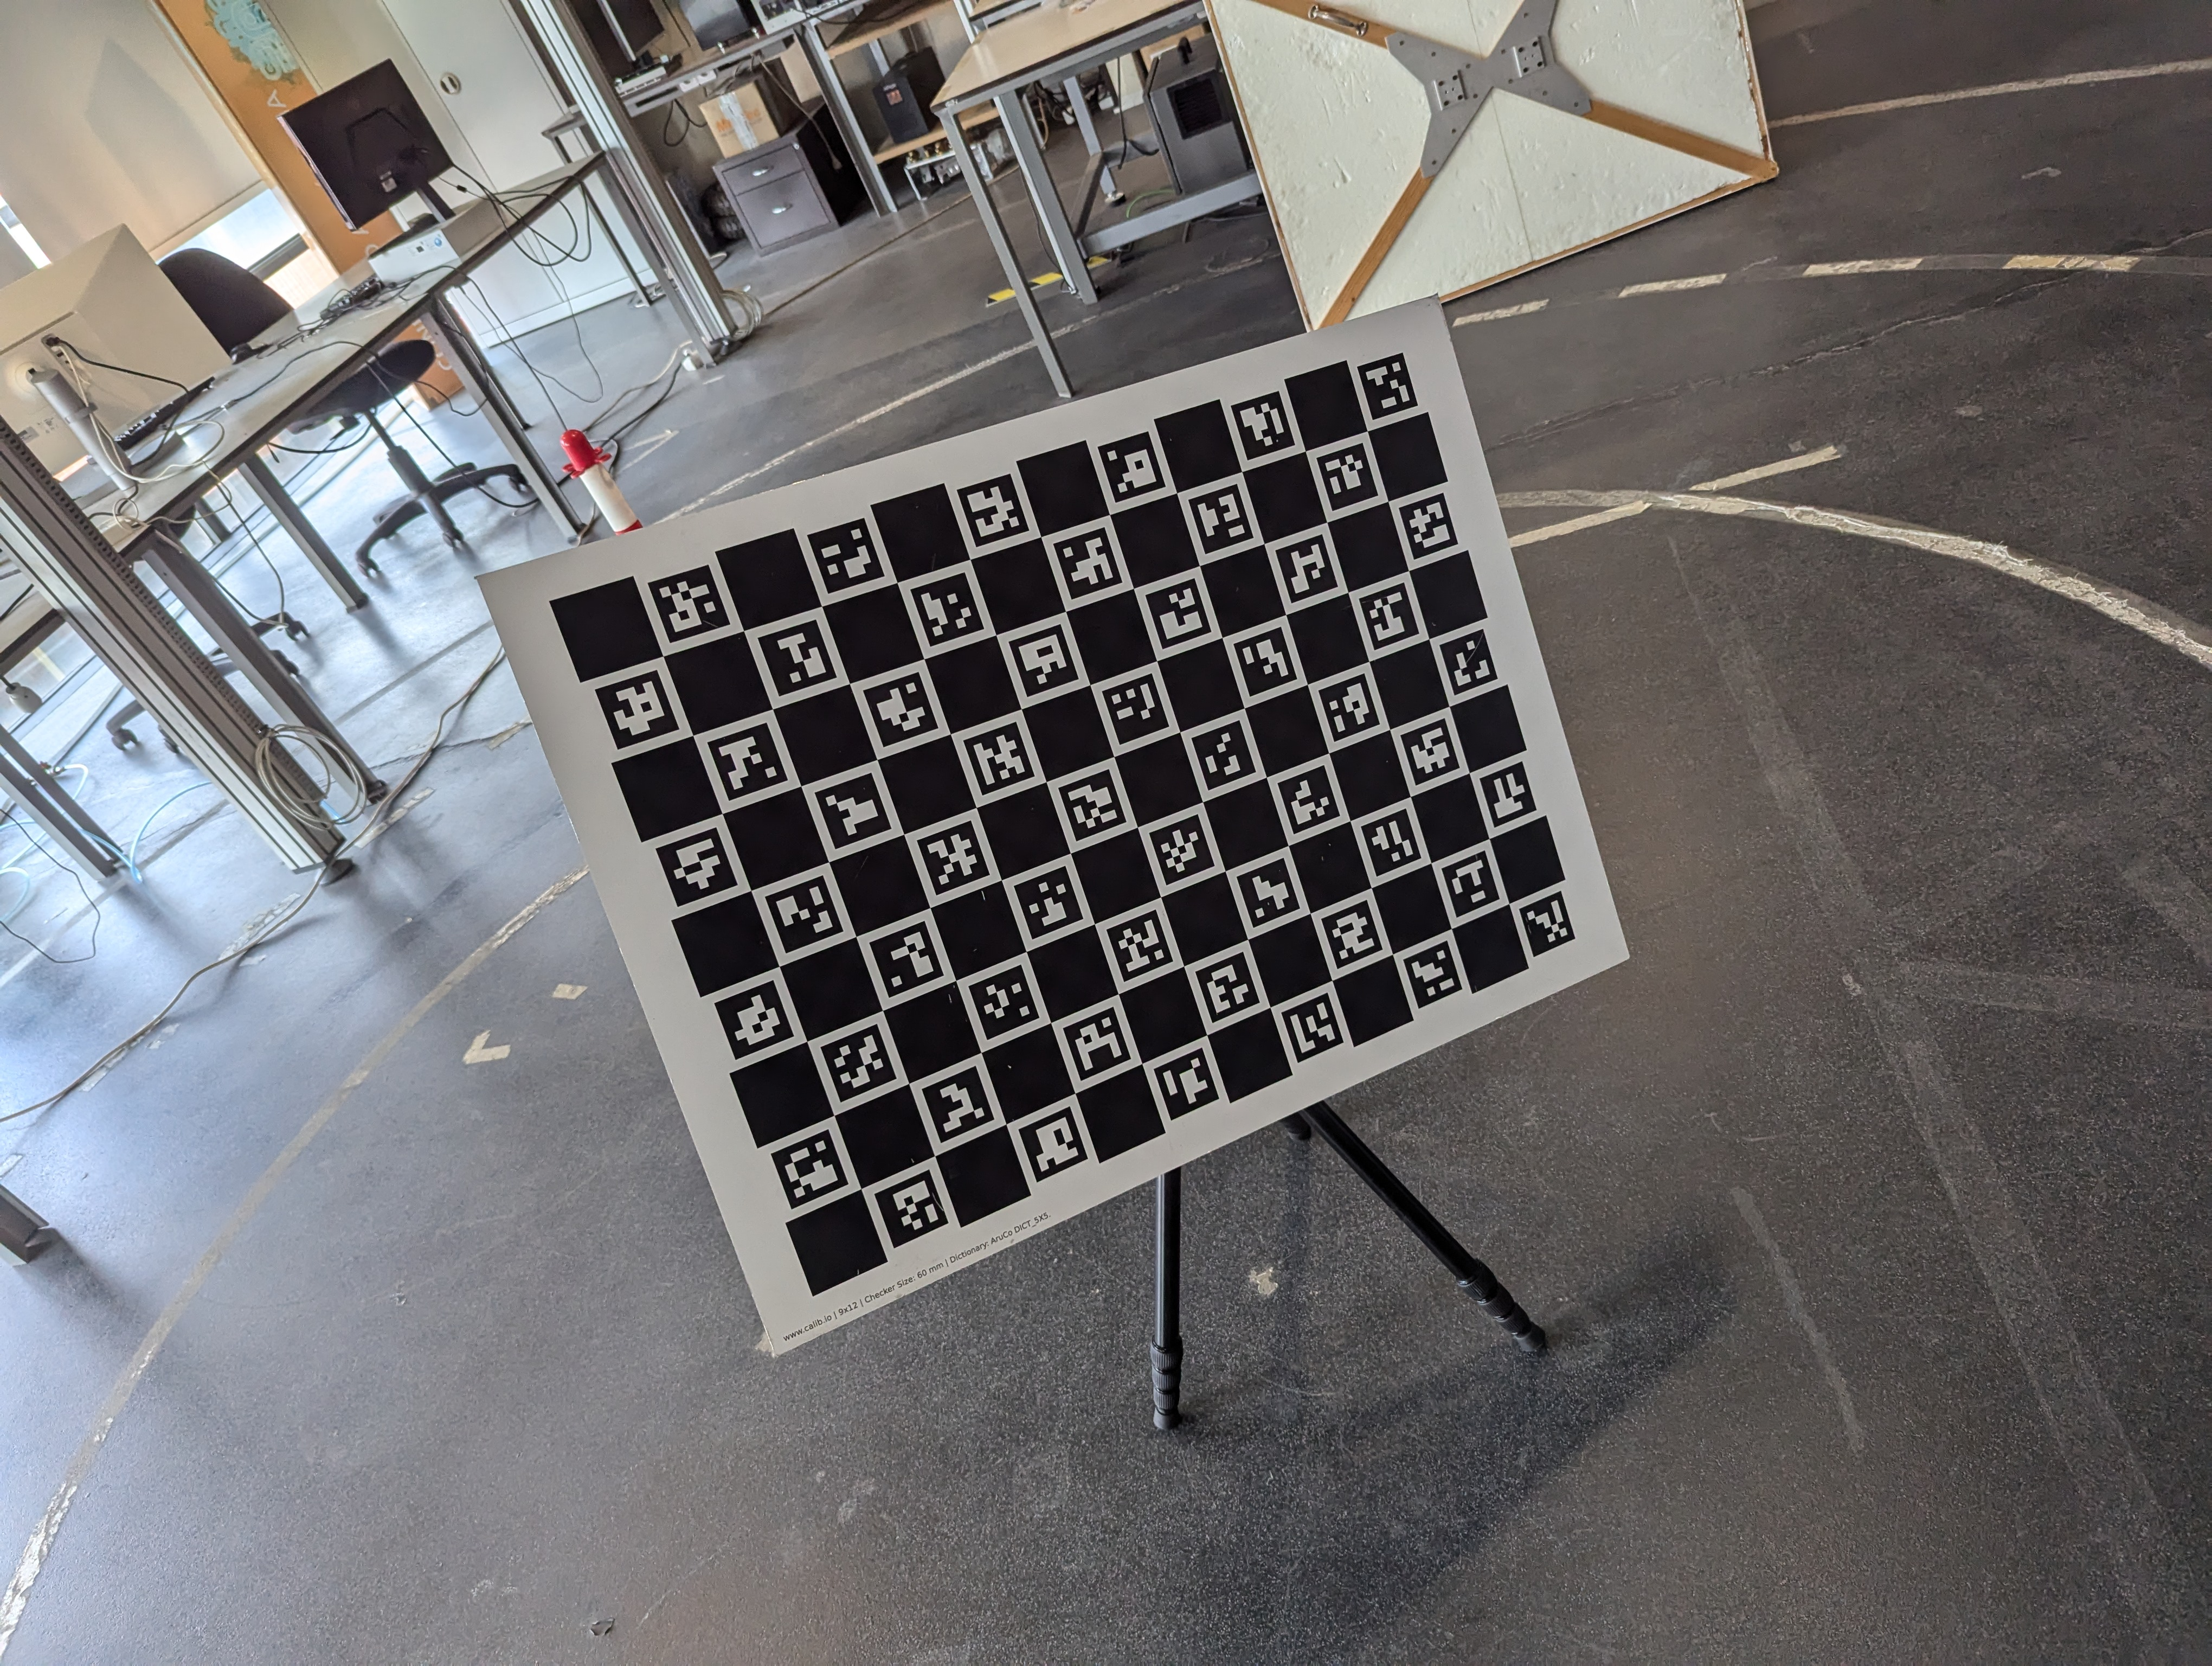
\includegraphics[width=0.8\linewidth]{resources/images/pattern_28.jpg}
    \caption{Example of an input image for the automatic labeler we aim to develop.}
    \label{fig:input}
\end{figure}

\begin{figure}[h]
    \centering
    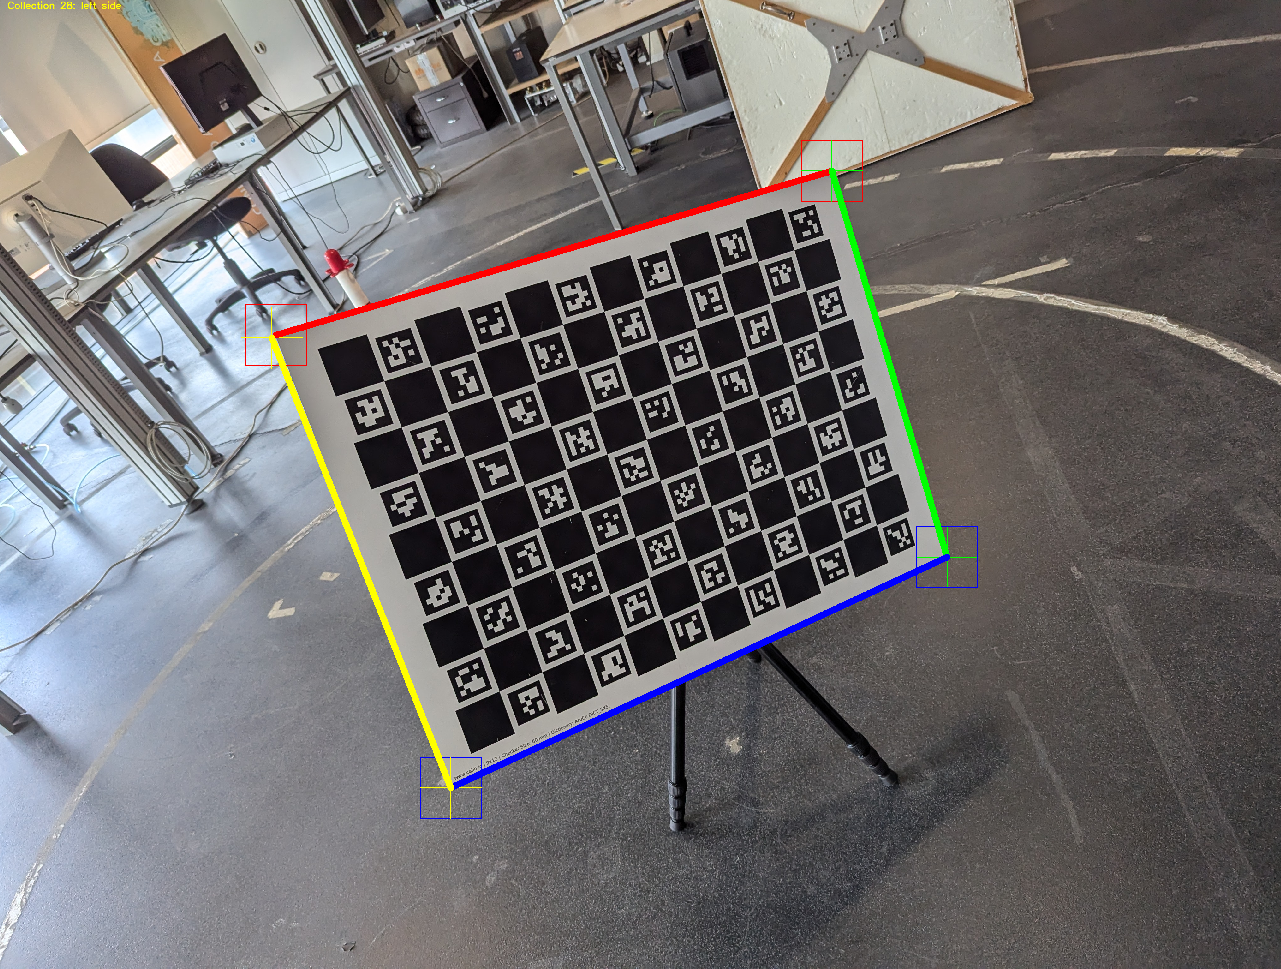
\includegraphics[width=0.8\linewidth]{resources/images/pattern_28_lines.png}
    \caption{Expected output from the automatic labeler, where the top border is marked in red, the right border in green, the bottom border in blue, and the left border in yellow.}
    \label{fig:output}
\end{figure}

\section{Abordagens}
\begin{frame}{Aquisição do dataset}
  
  \begin{columns}

    \column{0.4\textwidth}
      \begin{figure}[h]
          \centering
          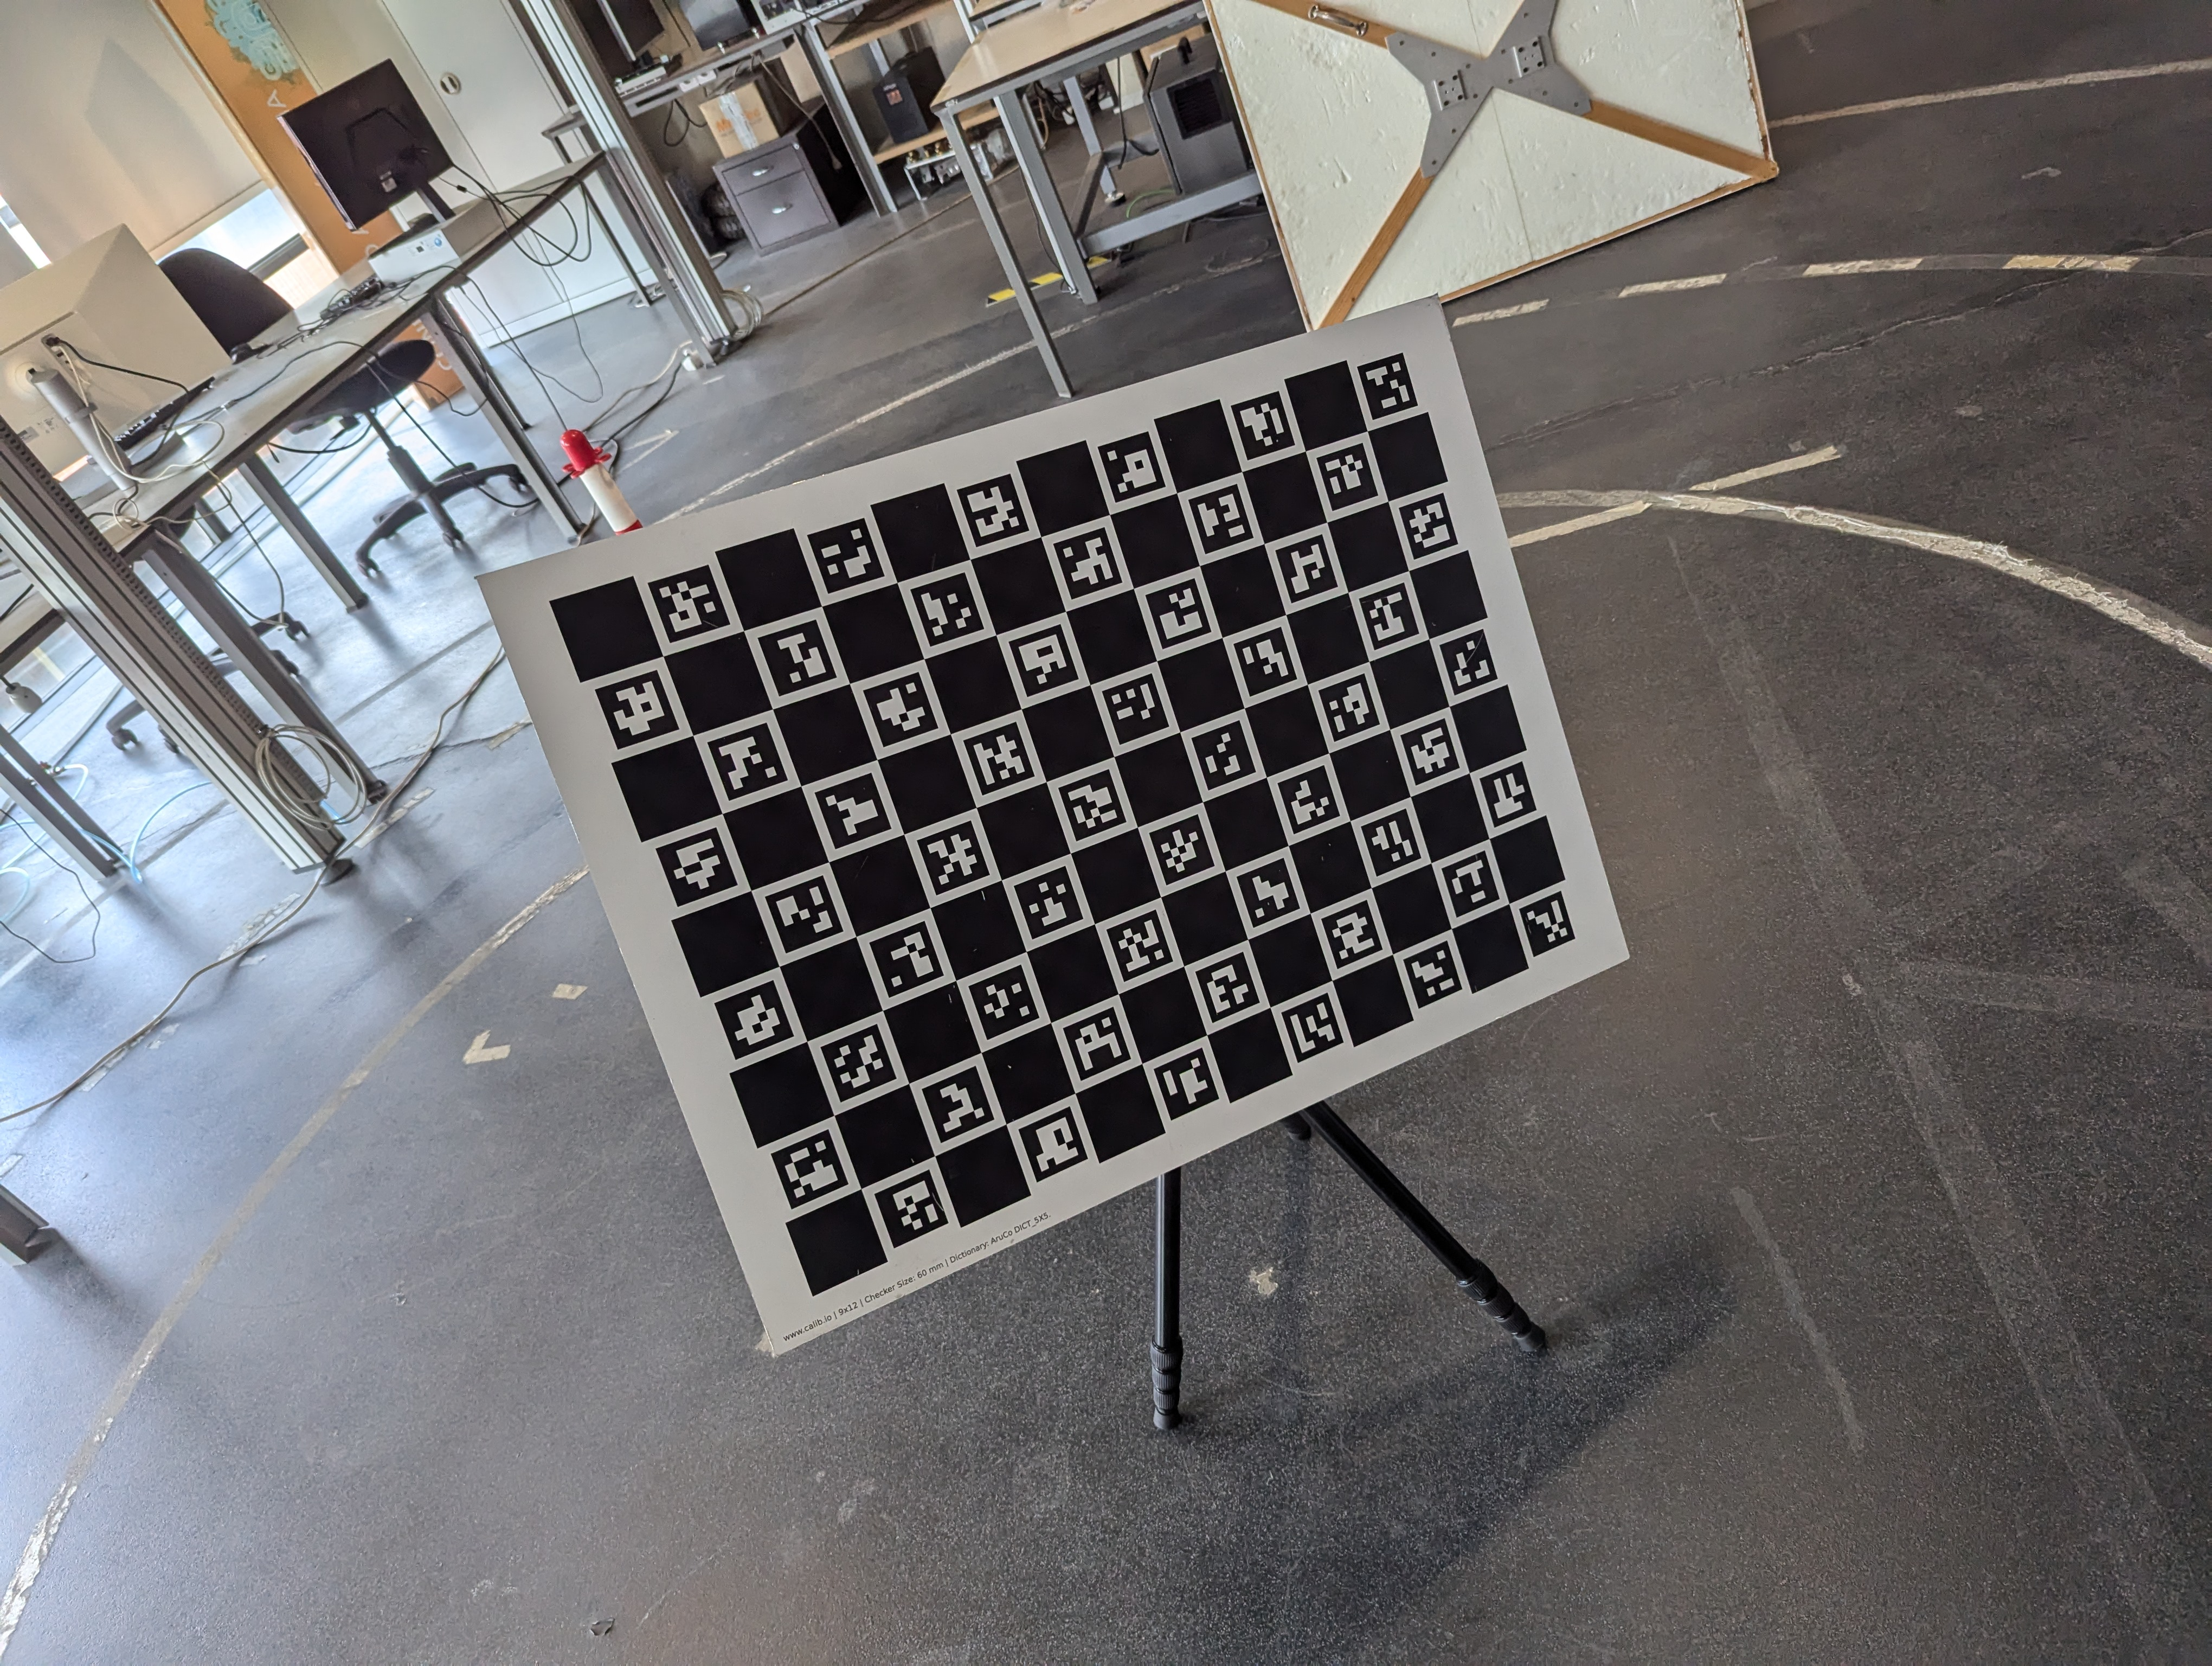
\includegraphics[width=0.9\textwidth]{resources/images/pattern_28.jpg}
          \captionsetup{labelformat=empty}
          \caption{Imagem original}
      \end{figure}
      % {\Huge\setstretch{1.0} Semântica\par}

    \column{0.4\textwidth}
      \begin{figure}[h]
          \centering
          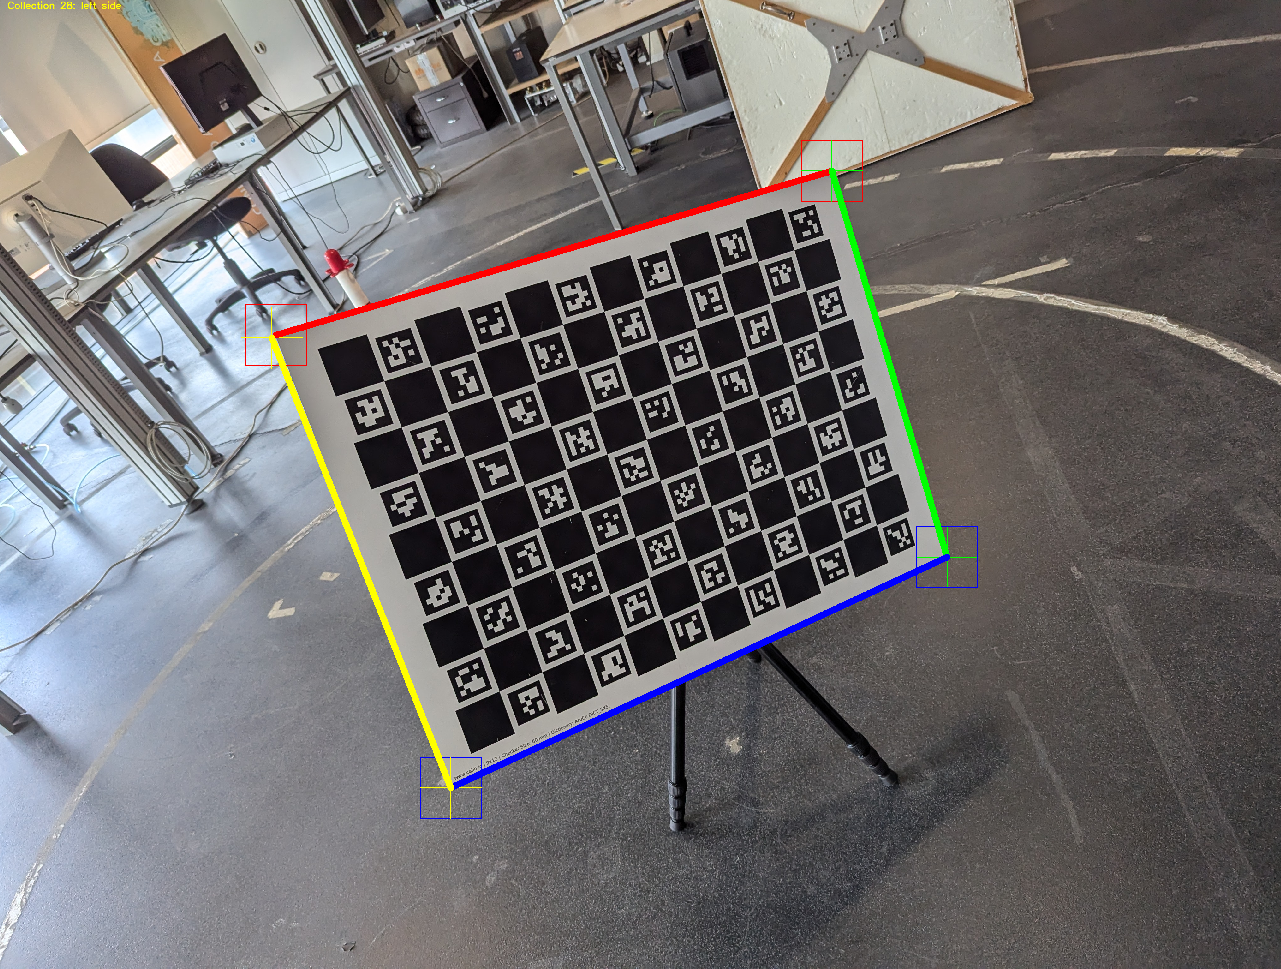
\includegraphics[width=0.9\textwidth]{resources/images/pattern_28_lines.png}
          \captionsetup{labelformat=empty}
          \caption{Anotações no ATOM}
      \end{figure}
  \end{columns}
      \vspace{\fill}
      \vspace{-0.2cm}


    % {\Huge\centering\setstretch{1.0} Panóptica\par}

      \begin{figure}[h]
          \centering
          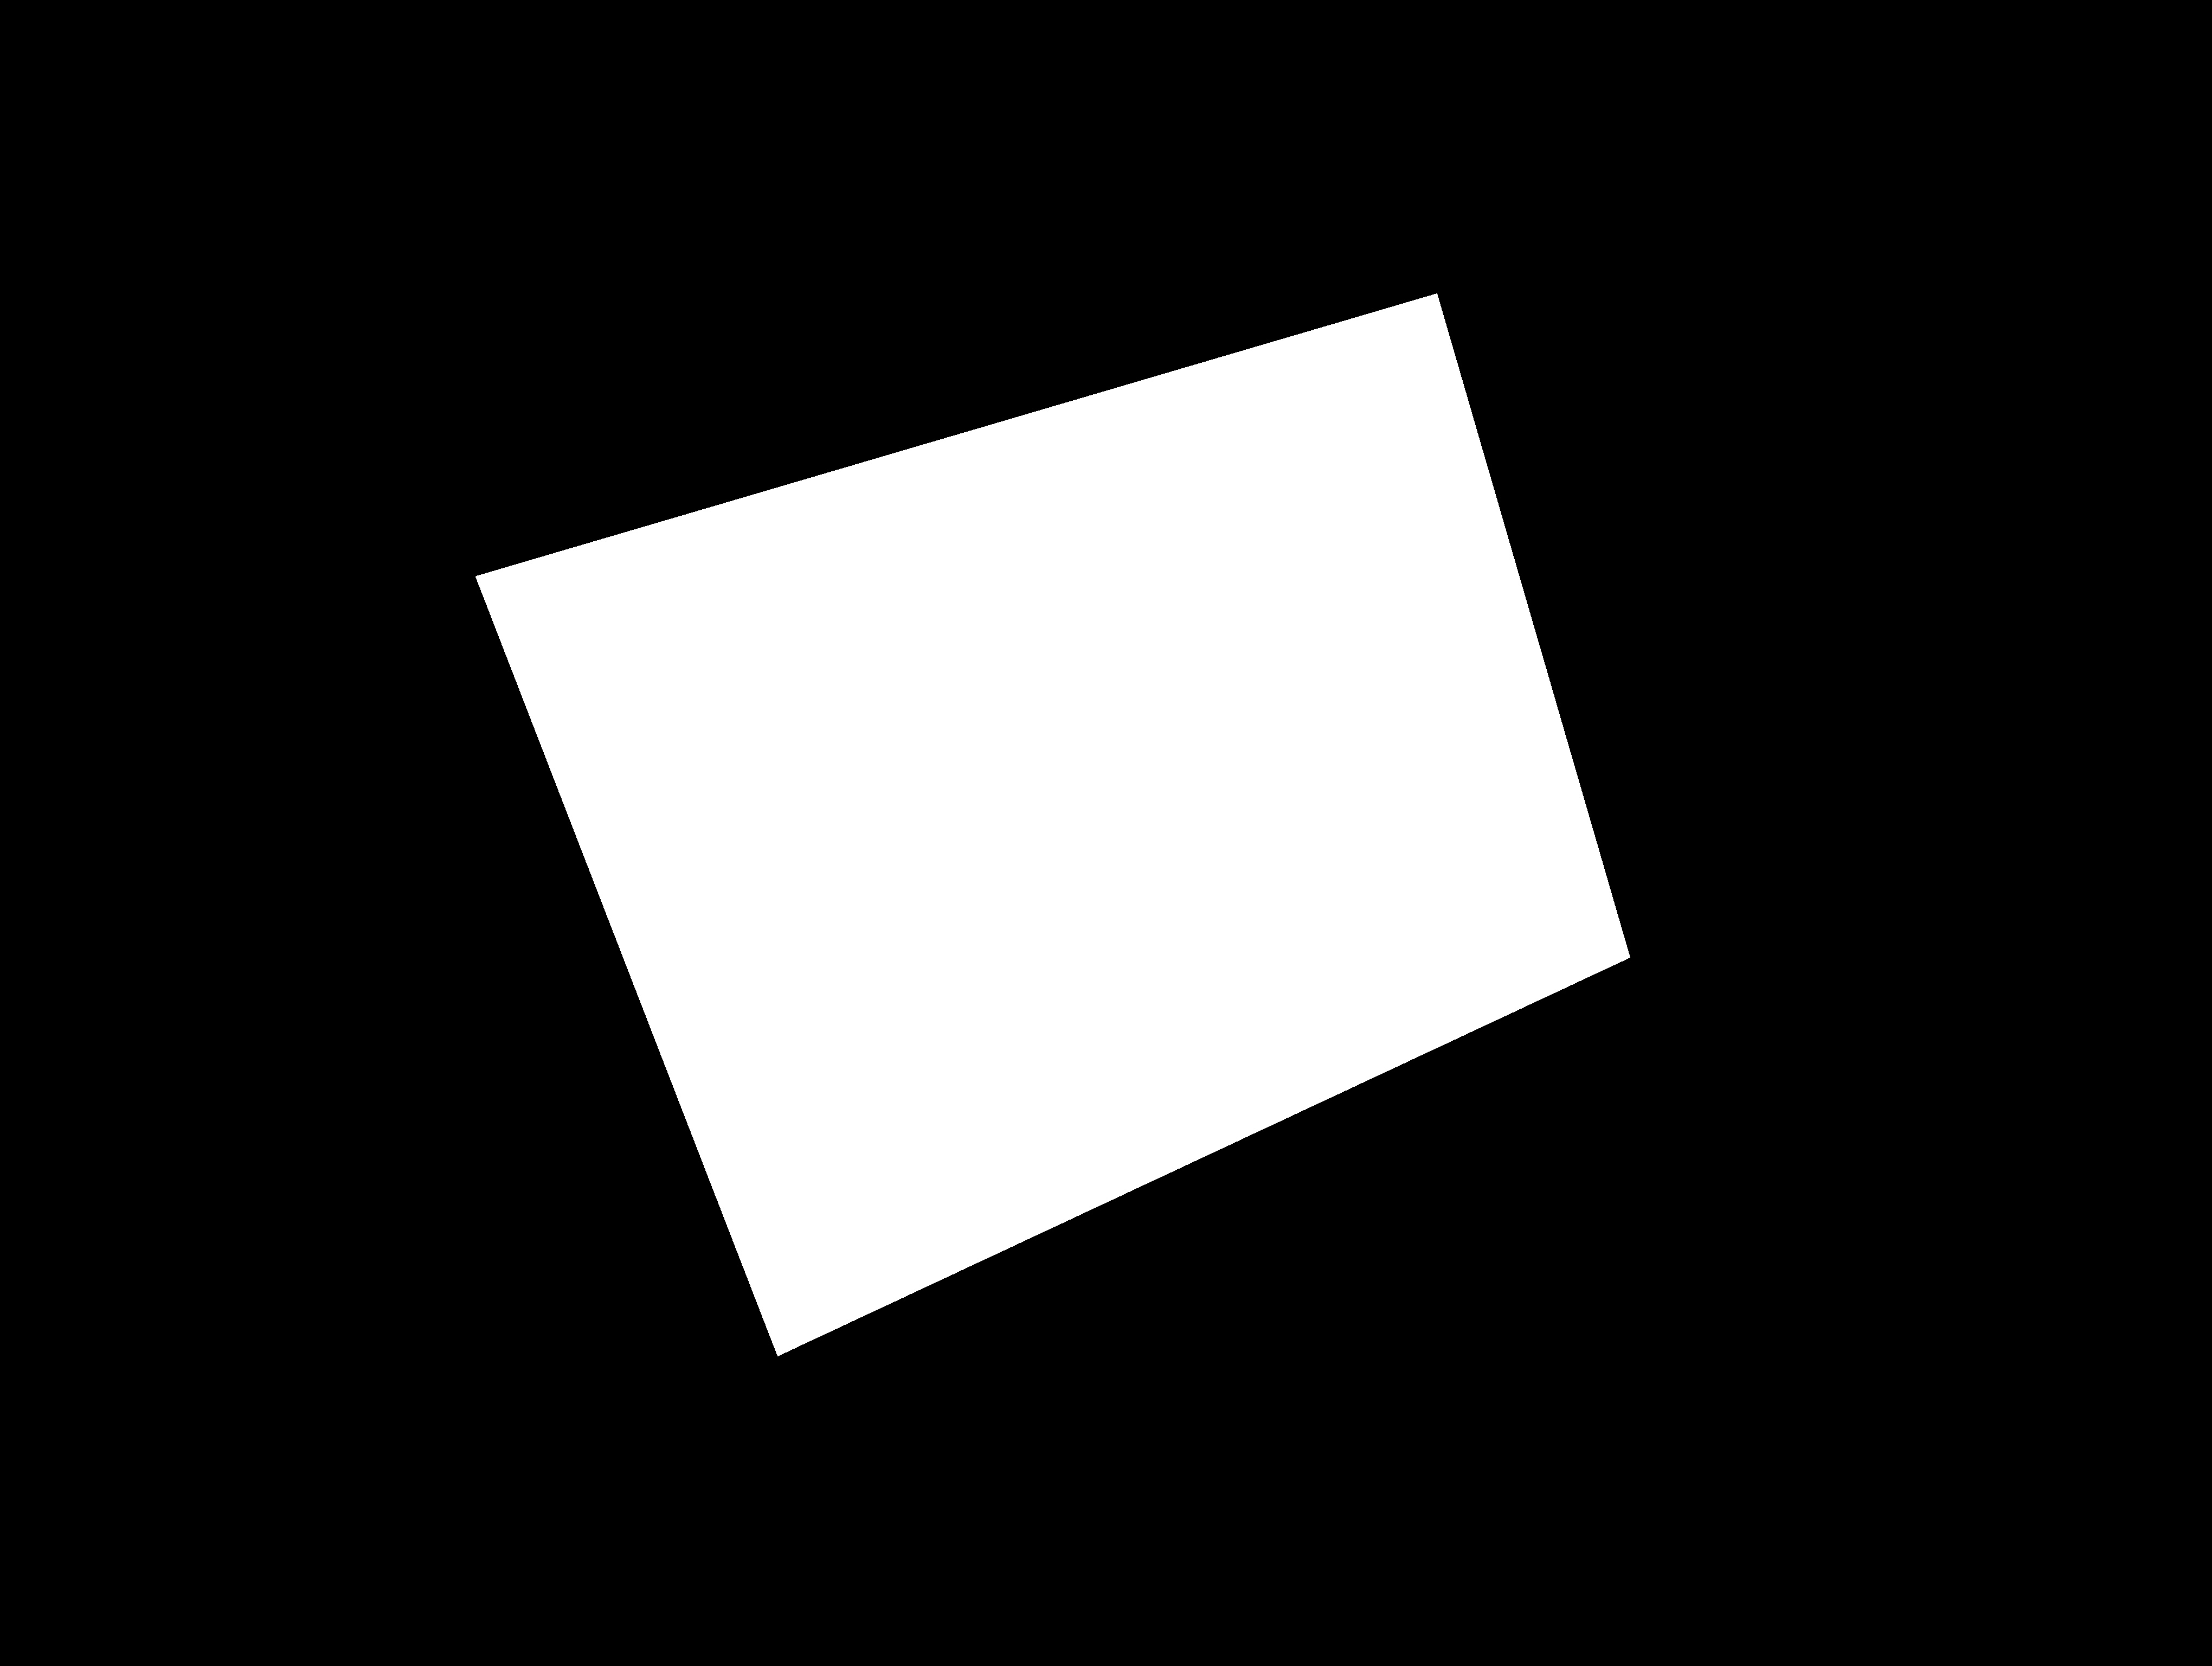
\includegraphics[width=0.36\textwidth]{resources/images/mask_pattern_28.jpg}
          \captionsetup{labelformat=empty}
          \caption{Conversão das linhas de contorno para uma máscara}
      \end{figure}
\end{frame}
\begin{frame}[c]{Seleção de modelos}{}

    \begin{itemize}
          \item Modelos pre-treinados do PyTorch
          \begin{itemize}
            \item DeepLabV3
            \item Fully Convolutional Network for Semantic Segmentation
            \item LRASPP
          \end{itemize}
          \item U-Net
    \end{itemize}

\end{frame}

\begin{frame}{Setup de treino}
  \begin{itemize}
    \item Loss function: Binary cross-entropy loss
    \item Optimizer: Adam
    \item Batch size: Máximo possível para a GPU
    \item 200 epocas por treino
  \end{itemize}
  
\end{frame}



\end{document}
